\chapter{Introduction}

\section{Background on gut microbiota: microbial ecosystems with important functions}

Trillions of microorganisms live on and inside the human body, with the highest densities being in the gastrointestinal tract \cite{the_human_microbiome_project_consortium_framework_2012}. Humans are not special: microbial communities have been found associated with macroorganisms across the entirety of the tree of life. Closer inspection of any of these host-microbe systems almost always reveals deeper connections than mere co-occurrence. Specific strains of bacteria are known to hide bobtail squid in moonlight with luminescence \cite{brennan_model_2014}, direct the formation of root nodules and nitrogen fixation in leguminous plants \cite{Teulet21758}, induce mating in single-celled eukaryotes \cite{woznica2017mating}, and much more. However, it is the relationship between humans and our gut microbes---collectively called gut microbiota---that has aroused the most scientific and popular interest in recent decades. 

This surge in interest is in large part due to unexpected interactions discovered between the gut microbiota and diverse aspects of human health and disease. Reviewing all of these interactions is beyond the scope of this work, but it is worth noting that beyond the more plausible functions of gut bacteria, such as aiding digestion \cite{Cox2014} and protecting against enteric infection \cite{McKenney2015}, the gut microbiota has been shown to regulate the immune system \cite{belkaid2014role}, alter developmental programs \cite{Troll2018}, modulate animal behavior \cite{sharon2019human}, and other surprising feats. Understanding how gut microbiota assemble, persist, and interact with their hosts therefore has major implications for both our basic knowledge of microbial ecosystems and therapeutic applications. 

Central to these problems are the notions of spatial organization and dynamics of bacterial populations within the gut. Organization in space and time is well-known to be important in determining species coexistence in macroscopic ecosystems \cite{tilman2018spatial, adlerGrass_2006}. Within the intestine, spatial organization and dynamics influence both the observed abundances of various bacterial species and how these populations interact with their animal hosts. To this end, the overarching goal of this dissertation work is to infer, through controlled experiments and quantitative analyses, rules that govern the spatial organization and dynamics of gut bacterial communities.

\section{Microbiota form: patterns of variation}

The notion that gut microbiota follow any semblance of rules at all, that they are anything but purely random collections of digesta, first appeared via large-scale surveys of the microbial species present at different body sites \cite{the_human_microbiome_project_consortium_framework_2012}. These studies revealed distinct patterns of variation incompatible with pure random sampling from the environment. Instead, we have the following picture: the gut microbiota is extremely dense and diverse. There are an estimated $10^{13}$ bacterial cells in the gut---roughly one for every human cell in the body \cite{sender2016revised}---comprising thousands of different species. This density is approximately 100 times higher than the density of a laboratory culture of E. coli grown overnight in nutrient-rich media. The gut microbiota assembles over the first $\sim$3 years of life, after which it becomes relatively stable in composition and measurably distinct from other peoples' \cite{the_human_microbiome_project_consortium_framework_2012,yassour_natural_2016}. The gut microbiota is unique to the gut, being easily distinguishable from environmental microbial communities, and even from microbial communities at different body sites \cite{the_human_microbiome_project_consortium_framework_2012}. For example, in terms of microbiota composition, my gut is almost certainly more similar to another person's gut than it is to my own mouth \cite{the_human_microbiome_project_consortium_framework_2012}. Summarized a bit more quantitatively, we can say that measures of dissimilarity between microbiota---for concreteness say a typical variance in species abundance---follows the following hierarchy \cite{fisher2017variable}:

\be
\Var_{\text{body sites}} \gg \Var_{\text{people}} \gtrsim \Var_{\text{time}}
\ee


In words: the variance across body sites within the same person is much greater than the variance across people at the same body site, which itself is usually greater than the variance across time within a single body site of a single person. This last inequality is not a strict one because although microbiota composition appears relatively stable over time in healthy adults, large fluctuations are observed in response to perturbations, such as antibiotic treatments or changes in diet \cite{dethlefsen2011incomplete,david_diet_2014,schlomann2019timescales}.

This hierarchy of variation immediately puts forth the notion that the assembly of gut microbiota is guided by some processes or factors that are not entirely random. If our intestines only did just sample from our local environment, we might expect the variance across people in different environments to exceed the variance across our own bodies. We also might expect that, as people travel about different environments, the variance over time might equal or exceed the variance between people even in the absence of large perturbations. Accounting for diet and other relevant factors, no trace of these types of geographical signatures have been found. We therefore conclude that there are likely intestine-specific rules governing gut microbiota composition that need to be inferred, and fundamental questions that need to be answered. Why are certain bacteria found preferentially in the gut? Why is one person's gut microbiota different from another's? What determines microbiota dynamics, both at baseline and in response to perturbation? After a decade of intense research efforts across the globe, these questions remain incompletely answered. 

Abstracting away the microbial community from the intestinal environment, these questions about patterns of variation and dynamics are the same ones that have been asked in the field of ecology for over a century. However, the sheer vastness of gut microbiota as ecosystems, combined with the staggering complexities of the human body, have resulted in a problem that challenges our understanding in new and formidable ways. While attempts to understand gut microbial communities in terms of just microbes and their interactions have been made \cite{bashan2016universality}, it is becoming increasingly clear that the context of the intestinal environment is paramount \cite{wiles2019other}. Indeed, the ordering of the variance hierarchy, with body site dominating, suggests that to understand how the gut microbiota works, one should peer into the gut itself and understand life there from the microbial point of view. This is the approach taken in this dissertation. 

\section{Microbiota form: spatial organization and dynamics}

Given the high density of bacteria in the gut ($\rho \sim 10^{11}$ cells/cm$^3$ $= 10^{-1}$ cells/$\mu$m$^3$  \cite{sender2016revised}), spatial structure is likely to be a key driver of bacterial population dynamics, and therefore microbiota composition. Indeed, a simple estimate suggests that most bacteria in the gut (typical size $\ell \sim  1$ $\mu$m) are closely packed, with a typical spacing $d \sim \rho^{-1/3} \sim 10^{1/3}$ $\mu$m, of order $\ell$. However, even a basic assessment of how gut microbes are organized spatially is lacking. The questions of \textit{why} they are organized the way that they are, and how this organization impacts dynamics, are even further from being understood.

These deficiencies are largely due to the hidden nature of gut microbiota. In most animals, it is extremely difficult to know which bacteria are where while the animal is still alive. In a notable recent paper \cite{zmora2018personalized}, healthy human subjects were invasively sampled at several points along the gastrointestinal tract, using a combination of endoscopy and colonoscopy, along with bacterial DNA sequencing. These measurements revealed distinct microbiota compositions at different anatomical sites, a finding that mirrored previous observations made in excised mouse intestines \cite{donaldson_gut_2015}. These patterns of composition along the length of the gut are likely driven, at least in part, by concurrent gradients in the chemical environment, including features like oxygen levels and pH \cite{donaldson_gut_2015}, though a causative relationship has not been rigorously established. In contrast, elegant experiments in a fluidic “gut-on-a-chip” system and mathematical modeling clearly demonstrated that intestinal fluid flow can reproduce observed patterns of increasing density of total bacteria along the gut, and can also, in combination with pH gradients, generate species-specific distributions \cite{cremer_effect_2016}.

Sequencing-based approaches have to date been limited to measuring microbiota spatial structure only on coarse scales, with maximum resolutions being around tens of centimeters for measurements along the length of the gut \cite{donaldson_gut_2015}. To probe length scales closer to that of bacteria themselves, histological methods have been developed and continue to be optimized for studying gut microbiota. In these experiments, typically done in mice, intestines are removed from sacrificed animals, treated with a fixative agent such as chloroform, embedded in paraffin wax, sliced into thin sections, and then subjected to various stains for visualizing bacteria and other intestinal features with optical microscopy \cite{tropini_gut_2017}. Through combinatorial labelling, it has been possible to simultaneously label up to 15 different bacterial strains in a mouse gut \cite{welch_spatial_2017}. These types of studies have shown that, in the large intestine, bacteria grow in dense clusters, with species mixing at scales down to the single-cell level, though larger clonal clusters of some species are observed \cite{welch_spatial_2017}. 

Histological approaches offer extremely high spatial resolution. However, the extensive processing involved in preparing the sample for imaging, including killing the animal and applying fixative, can generate serious artifacts and may alter bacterial community structure \cite{tropini_gut_2017}. In particular, loosely suspended contents in the fluid center of the gut are difficult to preserve. Older studies took a simpler approach of observing bacteria directly within human fecal samples \cite{van_der_waaij_vivo_1996}. These studies concluded that bacteria were largely encased in 3D mucus clusters, whose sizes spanned several orders of magnitude, and also implicated the immunoglobulin IgA in the formation of these structures, which has been further investigated in recent years \cite{moor_high-avidity_2017}. Even apart from artifacts induced by sample preparation, the high spatial resolution of both of these approaches comes at a cost of reduced scope: with fairly low throughput, it is difficult to assess larger-scale spatial patterns throughout the gut. 

Similar to studies of spatial organization, studies of gut microbiota dynamics are limited in resolution. Sequencing-based approaches using fecal samples as proxies of the intestinal environment have a maximum temporal resolution of around one sample per day \cite{schlomann2019timescales}. Long-term studies have shown that gut microbiota composition in healthy adults is relatively stable over years \cite{zoetendal_temperature_1998,rajilic-stojanovic_long-term_2013,caporaso2011moving}. In contrast, in response to antibiotics, the gut microbiota of healthy adults responds dramatically within the sampling period of a day \cite{dethlefsen2011incomplete}, indicating response dynamics on the scale of hours. Understanding how these timescales are connected is a major open problem \cite{schlomann2019timescales}. 

While histological methods enable bacteria-scale measurements of spatial organization, measurements of dynamics on the scale of bacteria---minutes and hours---are almost non-existent. Even a simple measurement of bacterial growth rate, routine practice for lab-cultured bacteria, is near impossible in most gut microbiota. Sophisticated metagenomic methods, which compare ratios of read counts from DNA sequencing near and far from the origin of replication on the bacterial chromosome, can track relative changes in growth rates, but converting these numbers to absolute rates is often not possible \cite{korem2015growth}. Alternatively, measuring the distribution of bacterial abundances over time in cohorts of sacrificed laboratory animals can lead to an effective growth rate, but without knowledge of additional processes, such as rates of bacteria entering and leaving the gut, or competition with other microbes, it is challenging to convert this number to an actual cell division rate. Arguably the most direct measurements of bacterial growth rate within an intestine are from the zebrafish system discussed here, where abundances are followed through time-lapse imaging \cite{jemielita_spatial_2014,wiles_host_2016,schlomann_sublethal_2019}. Summing the results of all these methods, we observe that bacteria replicate in the gut on scales ranging from once an hour to once a day. Beyond these timescales, the nature of bacterial dynamics in the gut remains underexplored.

\section{Connecting spatial organization and dynamics to microbiota function}

Important for this work, the spatial organization and dynamics of gut microbiota are likely critical to their function. Many interactions between gut bacteria and their animal host have found to be specific to particular bacterial strains \cite{wiles2020patterns}. Therefore, the dynamics of particular strain abundances likely impact host-bacteria interactions. In addition, how bacteria organize spatially in the gut can influence how they are sensed by the animal host. Bacteria that can access space close the epithelium lining of the gut, which is protected by the difficult-to-penetrate polymer gel of intestinal mucus, can present their molecular products more directly to the host than can other bacteria that are sequestered within the fluid center of the gut, known as the lumen \cite{johansson_gastrointestinal_2013,cullender_innate_2013,vaishnava_antibacterial_2011}. This process is known to occur with several bacterial pathogens \cite{chow_pathobionts_2011,gevers_treatment-naive_2014,kostic_microbiome_2014,carvalho_transient_2012}, where the ability to navigate to the epithelium is necessary for causing disease, but is less well-characterized for members of the resident microbiota. Further, the composition of animal cell types varies along the length of the gut \cite{lickwar_genomic_2017}, as does the composition of the microbiota \cite{donaldson_gut_2015}, so how bacteria are distributed longitudinally may also impact how they interact with the host. Together, these observations imply that a general understanding of gut microbiota spatial organization and dynamics will not only inform our ecological view of these systems, but may also uncover mechanisms underlying a variety of health and disease-related interactions.  


\section{Overview of experimental system: zebrafish, bacteria, and microscopy}

To address the gap in understanding of gut microbiota spatial organization and dynamics, I conducted live-imaging studies in larval zebrafish, a model vertebrate. In this section, I give a general overview of the experimental methods used in these studies. Methodological details are also included in each core chapter of this dissertation. 

\subsection{Zebrafish}
The zebrafish, \textit{Danio rerio}, has been a prominent model organism in biology, especially developmental biology, for several decades \cite{streisinger1981production}. First developed as a model at the University of Oregon, zebrafish have become a useful model becomes of their combined features of (1) being a vertebrate, thereby providing a high degree of similarity with human biology; (2) fast maturation times ($\sim$3 months) and high fecundity, which enables large-scale studies and screens; (3) the existence of powerful genetic tools for editing the zebrafish genome; and, most importantly, (4) optically transparent larvae, which allows for live imaging studies. Together, these features enable multicellular dynamics to be directly observed in their natural context, while simultaneously offering rigorous dissection of molecular mechanisms. 

In particular, in recent years zebrafish has emerged as a powerful model for host-microbe interactions, largely due to work conducted at the University of Oregon. A key milestone for this research was the development of protocols for deriving animals that are devoid of any microbes, or “germ-free”. Raising germ-free animals allows researchers to study the effects of having a microbiota, or none at all, on various aspects of host biology. Similar to mice and fruit flies, the absence of a microbiota is not lethal to zebrafish, but does lead to a variety of interesting differences, for example, in the composition of the immune system \cite{rolig_individual_2015}, in the proliferation of certain intestinal epithelial cells \cite{bates2006distinct}, and in the insulin producing capabilities of the pancreas \cite{Hill2016}. The details of the germ-free derivation process was reviewed in detail in \cite{melancon_best_2017}. This process involves sterilizing the surface of the embryo's chorion (a protective shell) with small amounts of bleach, iodine, and antibiotics, and then raising the animals in sterile media. Importantly, in current protocols for deriving germ-free zebrafish the animals are not fed, but subsist off of nutrients derived from their yolk sac. We raise germ-free fish in this way for a maximum of 7 days, after which nutritional deficiencies manifest.

In addition to studying the effects of a conventional microbiota versus no microbiota,  a germ-free animal offers the opportunity to assemble synthetic, model bacterial communities, consisting of a known set of species. Should a bacterial species be known to colonize zebrafish, it can be simply added to the aqueous environment of the fish flask, from where it enters the intestine likely through the mouth and esophagus. The work in this dissertation focuses almost exclusively on single species bacterial communities and how these populations interact with physical aspects of the intestinal environment. Focusing on a single species at a time allows isolation of interactions between bacteria and the host, avoiding complications arising from inter-species competition. 

\subsection{Bacteria}
All the bacteria studied in this work are species that are native to the zebrafish gut and were previously isolated. Recently developed genetic tools \cite{wiles_modernized_2018} have led to a large collection of zebrafish bacteria---around 10 species to date---that are engineered with fluorescent markers, enabling observation by fluorescence microscopy. These markers are fluorescent proteins, whose genes have been incorporated into the bacterial genome such that they are always expressed. These markers are extremely stable and do not interfere with normal bacterial physiology in any way measured to date. 

The ability to study bacteria that are native to zebrafish, as opposed to coming from another source, is extremely powerful. Specifically for the purposes of this work, by dissecting the strategies that these bacteria have evolved to thrive in the zebrafish gut (by design, the species that have been isolated and tagged are among the most abundant ones), we can better learn the rules that operate there. The process of becoming a dominant species in the zebrafish gut can be thought of as a puzzle that these bacteria have solved over the course of evolution. By understanding how these bacteria solved the puzzle, as opposed to a foreign bacteria that is colonizing a fish for the first time, we gain deeper insight into the workings of resident bacterial communities.

\begin{figure}%[h]
	\centerline{
		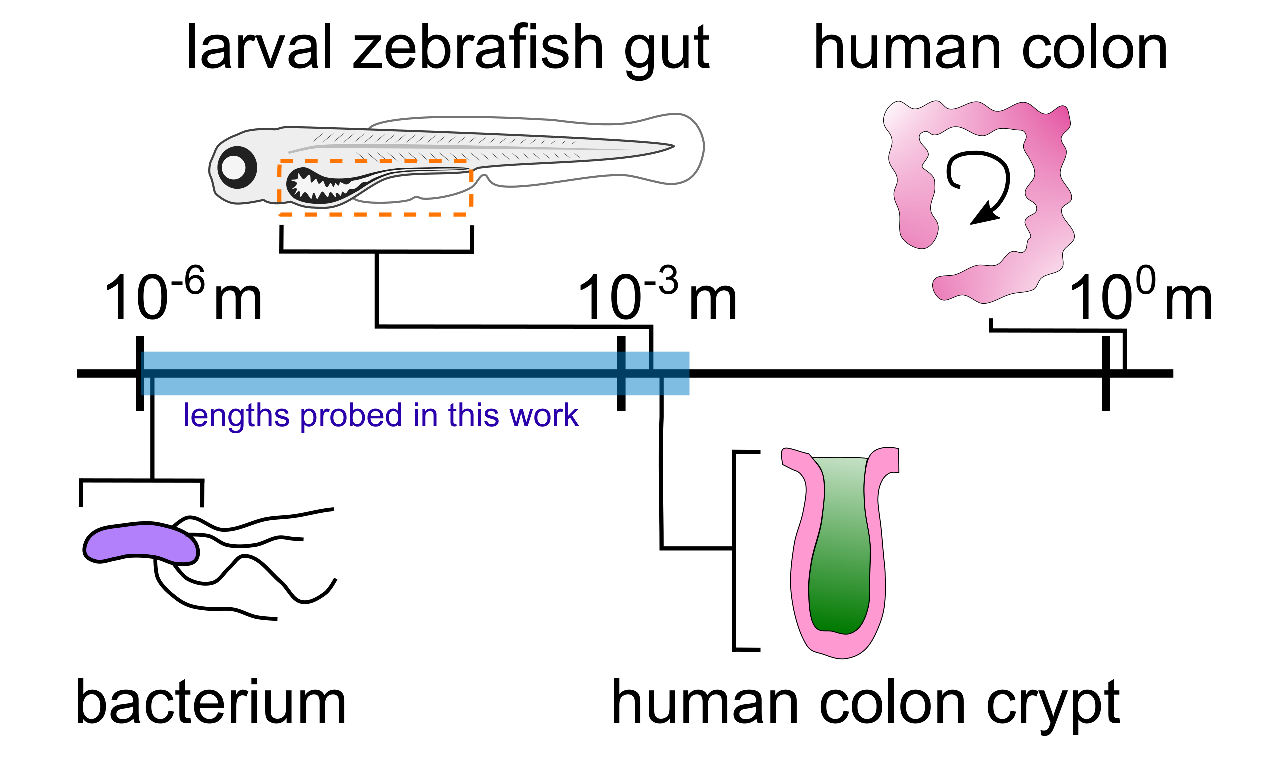
\includegraphics[width =6 in]{intro/intro_fig1.eps}}
	\caption{Summary of gut microbiota length scales.} {A bacterial cell (purple, shown with flagella) is approximately 1 $\mu$m long. A larval zebrafish, the model host organism for this dissertation work, has an intestine that is approximately 1 mm long (dashed orange box), which is large compared to bacteria, small compared to the length of the human gut ($\sim$1 m), but comparable to features of the human gut like colonic crypts. The length scales readily accessible by the microscopy techniques used in this dissertation work are highlighted in blue.}
\end{figure}

\subsection{Light sheet fluorescence microscopy}
Even with this ideal system of a transparent vertebrate host and fluorescent bacteria, imaging bacteria in the larval zebrafish gut is not trivial. The imaging system must simultaneously satisfy several technical requirements. First, the gut has rich three-dimensional structure, so we need to be able to acquire three-dimensional images. Second, there is a challenge of multiple length scales: the larval zebrafish intestine is approximately 1 mm long (the width narrows from $\sim$200 $\mu$m in the anterior to $\sim$70 $\mu$m in the posterior), which is small compared to human scales, but is large compared to bacteria (Fig. 1). To resolve individual bacteria and simultaneously study spatial patterns on the scale of the whole gut, we need to break up the full intestine into multiple, smaller three-dimensional fields of view, leading to a large number of images. Third, we need to acquire these images quickly because features in the gut move fast. The larval zebrafish gut contracts approximately twice a minute \cite{ganz_image_2018}, which would result in a blurred image if it occurred during image acquisition. Even more challenging are swimming bacteria, whose swim speeds can exceed 60 $\mu$m/s. Finally, because we want to do time-lapse imaging for several hours and study dynamics, we need to minimize photodamage during imaging, including the bleaching of fluorescent markers and phototoxic effects that arise in cells that are exposed to intense laser light. 

To simultaneously satisfy all of these requirements, I use a technique called light sheet fluorescence microscopy (LSFM) \cite{keller2008reconstruction,parthasarathy_monitoring_2018} LSFM is a type of fluorescence microscopy in which the excitation laser light is shaped into a thin sheet. Emitted light is captured on an axis perpendicular to this sheet, through a lens whose focal plane is matched to the light sheet plane. This unconventional geometry offers highly efficient light use, as regions of the sample away from the focal plane are not illuminated, minimizing photodamage. Moreover, with this geometry 3D images can be acquired rapidly by translating the sample perpendicularly through the sheet along this single axis. 

The axial resolution of a light sheet microscope is determined in large part by the sheet thickness. Due to the diffracting properties of Gaussian laser beams, there is a fundamental tradeoff between sheet thickness---and therefore axial resolution---and the field of view over which the sheet is roughly planar. Given a sheet of minimum thickness $w$ and wavelength $\lambda$, the characteristic length over which a sheet is planar is given by the Rayleigh length \cite{pedrotti2017introduction}, $\ell_R$,  for Gaussian beams:

\be
\ell_R = \frac{\pi w^2}{\lambda}.
\ee

Therefore, in designing a light sheet microscope for a given application the sheet thickness is chosen to optimize the balance between resolution and field of view. Since the larval zebrafish gut is fairly large, being $\sim$1 mm long, and we require resolution only on the scale of $\sim$1 $\mu$m to resolve individual bacteria, our microscope uses a somewhat thicker sheet, on the order of 3 um, which results in a Rayleigh length of $\sim$100 $\mu$m. In practice, the full gut is split into 4 regions which are imaged in sequence and then registered together computationally.

A light sheet microscope for imaging bacteria in the larval zebrafish gut was already constructed in the Parthasarathy lab when I began my dissertation research. My contributions to the optical and electronic systems were negligible. 

\section{Summary of core chapters}
This dissertation contains four core chapters. Chapter 1 describes a comparative study of bacterial spatial organization in the larval zebrafish gut across seven different bacterial species. It is discovered that the degree of bacterial aggregation, or “cohesion”, correlates strongly with localization along the length of the gut both across and within species, indicating the presence of general principles that govern spatial organization in the gut. 

Chapter 2 presents analytic calculations for a model of bacterial population dynamics in the gut. From previous work \cite{wiles_host_2016}, it was known that aggregated bacterial populations are susceptible to strong fluid transport up and down the intestine, with large aggregates occasionally being expelled from the gut altogether. These expulsion events register as large, abrupt, downward fluctuations in the local bacterial abundance within the gut. These fluctuations are modelled as stochastic, discontinuous jumps that arrive according to Poisson process. Coupling these jumps to conventional, deterministic logistic growth results in a piece-wise deterministic Markov process. Exact solutions for the model's stationary moments are derived and various limits are computed. These analytic results provide useful insight into how the dynamic processes of growth and stochastic expulsion generate the large variation observed in cross-sectional abundance measurements.

Chapter 3 investigates how bacterial aggregation behavior impacts the response of gut microbiota to low, sublethal levels of antibiotics. Such concentrations are frequently measured in the environment as the result of runoff from agricultural use, improper disposal in the medical sector, and pollution from manufacturing, but their impact on gut bacterial populations are poorly characterized. It is shown that low-dose antibiotics can enhance bacterial aggregation in vivo, which, when coupled to intestinal expulsion, leads to large, orders-of-magnitude reductions in bacterial abundances that are not predicted from in vitro responses. This effect is captured by a minimal kinetic model that connects in vivo antibiotic responses to sol-gel transitions in soft materials.

Finally, Chapter 4 takes a genetic approach to mechanistically study the role of bacterial swimming motility in host colonization. It is shown that swimming motility and chemotaxis enable bacteria to counter intestinal transport and maintain stable populations. An additional consequence of this bacterial lifestyle is that motile cells can stimulate strong immune responses around the gut, likely the result of swimming bacteria being able to access the epithelial boundary layer. Therefore, bacterial spatial organization, population dynamics, and intestinal inflammation are highly interconnected features of gut microbiota, and in this case are all largely determined by bacterial swimming motility. Through the use of inducible genetic switches that can toggle bacterial motility in situ, it is shown that all of these features can by dynamically controlled, indicating a potential application for precision microbiome engineering.

\section{A note on movie references}
Throughout this dissertation are references to supplemental movies that accompany figures and analyses. For simplicity, these movies can be accessed directly through the chapter's corresponding journal website, with the journal reference noted at the start of each chapter. 
